%!TEX program = lualatex
% One Philox-4x32 round as an engraved plate, for the FlexGEMM PTC 2026 deck.
% Vintage treatment follows ~/dotfiles/.ai/skills/creating-tikz-diagrams/vintage-style.md
% (typography/palette idea adapted from Foadsf/vintage-latex, CC BY-SA 4.0); the
% geometry and content are new. Paper matches the deck's Nuggets light paper.
% Build: latexmk -lualatex -interaction=nonstopmode -halt-on-error philox_round.tex
\documentclass[tikz,border=8pt]{standalone}
\usepackage{fontspec}
\usepackage{unicode-math}
\usetikzlibrary{arrows.meta,patterns,calc}
\setmainfont{EBGaramond}[
  Extension=.otf, UprightFont=*-Regular, ItalicFont=*-Italic,
  BoldFont=*-Bold, Numbers={OldStyle,Proportional}]
\setmathfont{Garamond-Math.otf}
\definecolor{paper}{HTML}{F4F0E8}
\definecolor{ink}{HTML}{2B241D}
\definecolor{amber}{HTML}{97551C}
% Transparent page: rasterize with pdftocairo -transp so the deck paper shows through.

\begin{document}
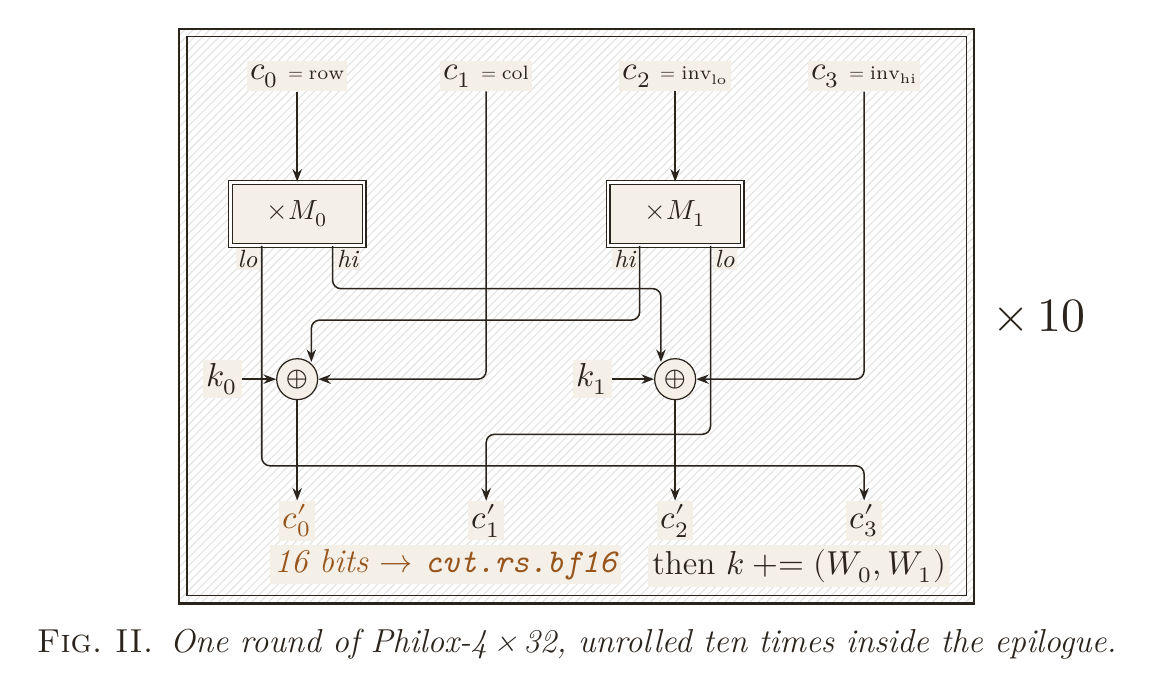
\begin{tikzpicture}[
  x=1cm, y=1cm, line width=.45pt, draw=ink, text=ink,
  flow/.style={draw=ink, line width=.55pt, -{Stealth[length=1.6mm,width=1.2mm]}},
  mul/.style={draw=ink, double, double distance=.9pt, minimum width=17mm,
    minimum height=8mm, fill=paper, inner sep=2pt},
  xor/.style={circle, draw=ink, fill=paper, minimum size=5.2mm, inner sep=0pt},
  lab/.style={font=\itshape\large, fill=paper, inner sep=1.2pt},
  tag/.style={font=\small\itshape, fill=paper, inner sep=.8pt},
]
  % Lane x-positions and levels; routing channels are explicit y levels.
  \def\xa{0} \def\xb{2.4} \def\xc{4.8} \def\xd{7.2}
  \def\ytop{0} \def\ymul{-1.4} \def\yxor{-3.5} \def\ybot{-5.3}
  \def\yhi{-2.35} \def\yhij{-2.75} \def\ylo{-4.2} \def\yloo{-4.6}

  % Plate with engraved hatching.
  \fill[pattern=north east lines, pattern color=ink!13] (-1.5,0.95) rectangle (8.6,-6.35);
  \draw[line width=.8pt] (-1.5,0.95) rectangle (8.6,-6.35);
  \draw (-1.4,0.85) rectangle (8.5,-6.25);

  % Inputs: the Philox counter is the output coordinate plus an invocation id.
  \foreach \x/\c/\m in {\xa/0/row, \xb/1/col, \xc/2/inv_{lo}, \xd/3/inv_{hi}} {
    \node[lab] (in\c) at (\x,\ytop+0.35) {$c_{\c}$\;\scriptsize$=\mathrm{\m}$};
  }

  % Multiply boxes (32x32 -> 64 bits: hi and lo words) and XOR junctions.
  \node[mul] (m0) at (\xa,\ymul) {$\times M_0$};
  \node[mul] (m1) at (\xc,\ymul) {$\times M_1$};
  \node[xor] (x0) at (\xa,\yxor) {$\oplus$};
  \node[xor] (x2) at (\xc,\yxor) {$\oplus$};
  \node[lab] (k0) at (-0.95,\yxor) {$k_0$};
  \node[lab] (k1) at (3.75,\yxor) {$k_1$};

  % Outputs.
  \node[lab, text=amber] (o0) at (\xa,\ybot) {$c_0'$};
  \node[lab] (o1) at (\xb,\ybot) {$c_1'$};
  \node[lab] (o2) at (\xc,\ybot) {$c_2'$};
  \node[lab] (o3) at (\xd,\ybot) {$c_3'$};

  \draw[flow] (in0) -- (m0);
  \draw[flow] (in2) -- (m1);

  % Feistel wiring, orthogonally routed with small rounded corners.
  \begin{scope}[rounded corners=3pt]
    \draw[flow] ($(m0.south)+(0.45,0)$) |- (4.62,\yhi) -- ($(x2.north)+(-0.18,-0.05)$);
    \draw[flow] ($(m1.south)+(-0.45,0)$) |- (0.18,\yhij) -- ($(x0.north)+(0.18,-0.05)$);
    \draw[flow] ($(m1.south)+(0.45,0)$) |- (\xb,\ylo) -- (o1.north);
    \draw[flow] ($(m0.south)+(-0.45,0)$) |- (\xd,\yloo) -- (o3.north);
    \draw[flow] (in1.south) |- (x0.east);
    \draw[flow] (in3.south) |- (x2.east);
  \end{scope}
  \node[tag, anchor=north west] at ($(m0.south)+(0.47,-0.02)$) {hi};
  \node[tag, anchor=north east] at ($(m0.south)+(-0.47,-0.02)$) {lo};
  \node[tag, anchor=north east] at ($(m1.south)+(-0.47,-0.02)$) {hi};
  \node[tag, anchor=north west] at ($(m1.south)+(0.47,-0.02)$) {lo};
  \draw[flow] (k0) -- (x0.west);
  \draw[flow] (k1) -- (x2.west);
  \draw[flow] (x0) -- (o0);
  \draw[flow] (x2) -- (o2);

  % Repetition, key schedule, and the one output word we use.
  \node[font=\LARGE, anchor=west] at (8.7,-2.7) {$\times\,10$};
  \node[font=\large\itshape, anchor=north west, text=amber, fill=paper, inner sep=1.5pt]
    at (\xa-0.35,\ybot-0.3) {16 bits $\to$ \texttt{cvt.rs.bf16}};
  \node[font=\large, anchor=north east, fill=paper, inner sep=1.5pt]
    at (8.3,\ybot-0.3) {then $k \mathrel{+}= (W_0,W_1)$};

  % Caption.
  \node[anchor=north, font=\large] at (3.55,-6.55)
    {\textsc{Fig.\ II.}\enspace\textit{One round of Philox-4\,{\texttimes}\,32, unrolled ten times inside the epilogue.}};
\end{tikzpicture}
\end{document}
